\begin{figure}[ht]\centering
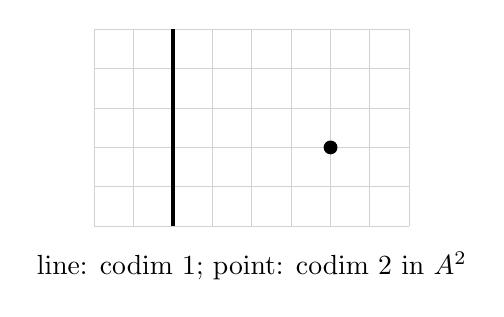
\begin{tikzpicture}
\draw[step=.5,gray!35] (0,0) grid (4,2.5);\draw[very thick] (1,0)--(1,2.5);\fill (3,1) circle (2.5pt);
\node at (2,-.5) {line: codim $1$; point: codim $2$ in $\mathbb A^2$};
\end{tikzpicture}\caption{Codimension distinguishes a divisor-like line from a closed point.}\label{fig:vi31-09}\end{figure}